\documentclass[11pt, a4paper]{article}
\usepackage[utf8]{inputenc}
\usepackage[T1]{fontenc}

\usepackage{tikz}

\begin{document}
    
\begin{center}
    {\Huge{Hello!}}\\
    So this is a Ti\textit{k}Z tutorial for newbies.
\end{center}

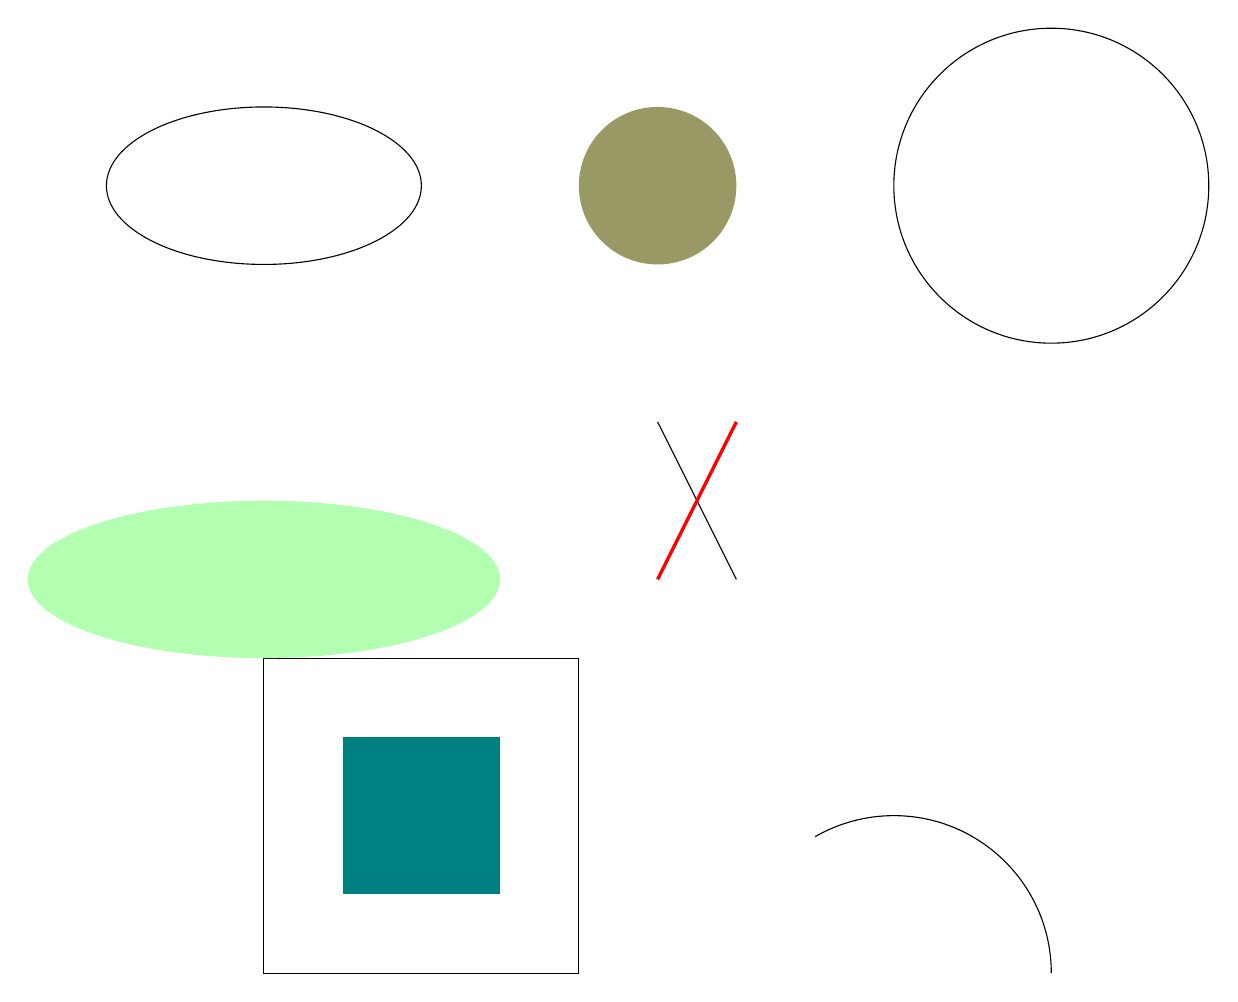
\begin{tikzpicture}
    \draw (5, 7) -- (6,5);
    \draw[red, very thick] (5, 5) -- (6,7);
    \draw (0, 0) rectangle(4, 4);
    \draw (10, 10) circle(2cm);
    \draw (0, 10) ellipse(2cm and 1cm);
    \draw (10, 0) arc(0:120:2cm);
    
    \fill[teal] (1, 1) rectangle(3, 3);
    \fill[blue!40!yellow] (5, 10) circle(1);
    \fill[green!30] (0, 5) ellipse(3 and 1);
\end{tikzpicture}


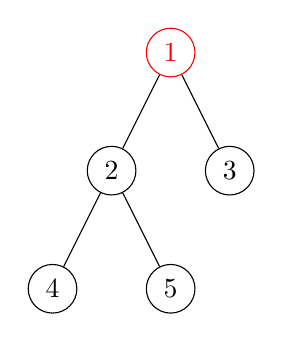
\begin{tikzpicture}[every node/.style={circle, draw=black}]
    \node[red]{1}
        child { node{2}
            child {node{4}}
            child {node{5}}
        }
        child {node{3}}
    ;

    
\end{tikzpicture}

\tikzset{
    treenode/.style={align=center, inner sep=0pt},
    % Black nodes
    node_black/.style={treenode, circle, white, font=\bfseries, draw=black, fill=black,
                    text width=0.8cm},
    % Red nodes
    node_red/.style={treenode, circle, red, very thick, text width=0.8cm},
    % Nil nodes
    node_nil/.style={treenode, rectangle, fill=black, minimum width=0.3cm, minimum height=0.3cm}
}

\begin{tikzpicture}[->, level/.style={sibling distance=2cm, level distance=1.5cm}]
    \node[node_black]{38}
        child{ node[node_red]{19}
            child{ node[node_black]{12}
                child{ node[node_red]{8} }
                child{ node[node_nil]{} }
            }
            child{ node[node_black]{31} }
        }
        child{ node[node_black]{41} }
    ;
    
\end{tikzpicture}
\end{document}